\chapter{Proposed approach}
\label{chap:proposed_approach}
	\textit{This chapter displays the problems as well as the malicious request validator's input and output. Then we offer the design and architecture of the problem's solutions.}
\minitoc

\section{Cyber security problems}
\label{Cyber problems}
WAFs, as previously indicated, are frequently used, however, they suffer from high FP. We aim to enhance the accuracy of WAFs, using the help of machine learning rather than rule-based approaches.  \\
Because WAFs only cover the Application Layer, the network requests are the model's input (mostly HTTP requests). Our methodology produces the same result as WAFs: whether the request is malicious or not.\\
With its nature, WAF is obligated to have fast processing speed in deciding whether an incoming request is reliable or not. For user experiences, we can't examine the request's veracity for minutes before granting or denying access. Our system's time constraint must be in milliseconds.\\
Any flaw in an organization's internal controls, system procedures, or information systems is known as a vulnerability in cyber security. Cybercriminals may target these vulnerabilities and exploit them through the points of vulnerability.
These hackers can enter the networks without authorization and seriously harm data privacy. As a result, it is crucial to constantly check for cybersecurity vulnerabilities because flaws in a network could lead to a complete compromise of an organization's systems.
Let's take a look at some common cybersecurity vulnerabilities\footnote{
    Intellipaat. \textit{What is Vulnerability in Cyber Security? Types and Definition}.
    Mar 2023.
    \url{https://intellipaat.com/blog/vulnerability-in-cyber-security/}
}:
\begin{itemize}
    \item \textbf{Zero-day vulnerabilities}
    Zero-day vulnerabilities are specific software flaws that the attackers are aware of but that a company or user hasn't yet discovered.
    Since the vulnerability has not yet been identified or reported by the system manufacturer, there are no known remedies or solutions in these situations. These are particularly risky because there is no protection against them before an attack occurs. To reduce the risk of zero-day attacks, it is crucial to exercise caution and constantly check systems for vulnerabilities.
    \item \textbf{Poor Encryption}
    If a network has weak or nonexistent encryption, it will be easier for attackers to intercept system communications and compromise them. Cybercriminals may obtain crucial information and introduce misleading information onto a server when there is weak or unencrypted data. This may result in regulatory body fines and adversely jeopardize an organization's efforts to comply with cyber security regulations.
    \item \textbf{System misconfigurations}
    System failures can be caused by network assets with inappropriate security settings or restrictions. Networks are frequently searched for system errors and vulnerable spots by cyber criminals. Network misconfigurations are increasing as a result of the quick digital revolution. Working with knowledgeable security professionals is crucial when implementing new technology.

\end{itemize}
\section{Designs}
\label{design}
To summary, numerous strategies for identifying malicious URLs have been proposed. Most of these solutions utilize supervised-based machine learning techniques for classification. This technique can detect irregularities between requests, but it cannot extract these abnormalities into human-readable form in order to reconstruct the WAF. Relying solely on machine learning eventhough brought higher accuracy like in \cite{s22093373}, WAFs need to be time-efficient. We can not compromise accuracy for speed, hence these methods don't work for WAFs.\\
We come to the approach is to categorize the incoming request and analyze its structure, with moderate reliability, then combining the result of these two process to achieve the high precision yet does not expending an excessive amount of time.

We have some theses to prove why we decide to design in this way: \\
\textbf{Thesis 1}
In his 1996 paper, The Lack of A Priori Distinctions Between Learning Algorithms, D. H. Wolpert introduced the No Free Lunch theorem for supervised machine learning and stated a quote at the beginning of his paper. The theorem states that given a noise-free dataset, “for any two machine learning algorithms A and B, the average performance of A and B will be the same across all possible problem instances drawn from a uniform probability distribution.” This means  “an algorithm may perform very well for one problem, but that gives us no reason to believe it will do just as well on a different problem where the same assumptions may not work.” \\
\textbf{Thesis 2}
Moreover, simpler models like logistic regression have more bias and tend to underfit, while more complex models like neural networks have more variance and tend to overfit. \\
\textbf{Strengths and Weaknesses of Logistic Regression:} 
Let's take a look at some advantages provided by Logistic Regression. Firstly, it's easy to deploy, and it calculates accurately and fasts with big data. Secondly, it can handle both continuous and discrete data. Next, it's suitable for binary or multiclass classification problems. Finally, it allows us to determine the importance of input features. Besides the strengths, this model also has some weaknesses.
First, this model cannot deal with data that is non-linear or has complex linear relationships. Second, it is sensitive to noise and outliers in data. Next, it can only be applied to classification problems, not to unsupervised learning algorithms. Lastly, it is prone to overfitting when the number of features is larger than the number of training samples.

\textbf{Strengths and Weaknesses of CNN:} 
CNN model combined with word2vec is a widely used method in Machine Learning to perform natural languages processing tasks such as text classification or machine translation. Below is a detailed analysis of the strengths and weaknesses of the CNN model combined with word2vec.
Let's look at some of the CNN model's benefits. First, it can handle ordered data, including long data strings. Second, it can remember past information and apply it to future decisions. Next, it helps machine learning models understand the meaning of words and sentences in natural language. Another advantage, this model is capable of learning common features from texts, resulting in better prediction results with never-before-seen new text. Finally, CNN is faster by design compared to RNN - the more fitting model to categorize text. This machine learning model also has some weaknesses. The first one is that the CNN model requires a lot of computational resources to train due to many parameters. The following disadvantage is that sometimes it is not effective for problems with complex structured data such as images. Next, it is necessary to use appropriate dictionaries to represent words in vector space. Eventually, it is difficult for it to deal with words that are not in the user dictionary. 

\textbf{Thesis 3}
Ensemble learning is an approach that combines diverse models to improve performance. The idea behind integrating different models is logical: each model has unique abilities, and when combined, they may excel in multiple tasks or subtasks. When these models are appropriately merged, they create a potent training algorithm capable of enhancing overall performance compared to using individual models alone.
Ensemble learning reduces variance and bias, improving predictions of the developed model. Technically speaking, it helps avoid overfitting.

This problem classifies the input data as yes/no. It needs accuracy and the data set is not large, needs high accuracy. So we decided to combine logistic regression and CNN model.



\subsection{Architecture}
\label{architecture design}
\subsubsection{Data exploration and Sanitization}
\label{data preprocessed}
Our goal is to classify request supplied as inputs in order to determine whether they are harmful or inoffensive. The sample of request data consists of different categories including: 
\begin{itemize}
    \item \emph{Plain text:} request that contains data but does not trigger any machine execution, typically in the form of HTML, JSON, XML, and CSV, etc.
    \item \emph{Client-side script:} request in form of programming languages or scripts that can be executed on client's machine
    \item \emph{Server-side script:} request in the form of programming languages (mostly back-end programming languages like PHP, JAVA, PYTHON, and so on) that can change the behavior of the application or web
    \item \emph{Shell script:} request in the form of shell scripts that can run jobs on the server or change the server's or operating system's behavior
    \item \emph{SQL script:} request that in form of SQL, can be used to query data from the database.
\end{itemize}
 The textual data acquired in the previous phase is going to be cleaned and standardized. To minimize feature complexity and improve classification performance, the request was preprocessed by eliminating symbols and punctuation. The text data collected will be transformed to lower case and then normalized. The goals of the normalization procedure were dual. First, the text must be converted from unstructured data to a structured word vector. Second, by deleting unneeded words and decreasing the number of words by roots them to their originals, we may reduce the scarcity of feature vectors.
However, malicious attacker usually use methods like slight modification to make an imposter URL or request looks legitimate, we skip severals step in conventional Natural Language Processing: 
\begin{itemize}
    \item Removing stop word
    \item Stemming (the process of reducing infected words to their stem)
    \item Lemmatization (returning to the base form of the words...)

\end{itemize}
\subsubsection{Model Selection and applying Natural language processing}
\label{NLP}
Because four of the five categories are structured languages, we must first create a special tokenizer to map the request into a defined set of keywords (client-side script, server- side script, and SQL script).
To convert the words (the tokens) to their numerical equivalents, a corpus containing a list of unique tokens based on their frequency of occurrence in each class was created. To put it in more formal mathematical terms, the TF-IDF score for the word t in the document d from the document set D is calculated as follows:
\begin{align}
    tf\:idf(t,\: d,\: D)\; =\; tf (t,\: d) \; . \; idf (t.\: D)
\end{align}
Where: 
\begin{align}
    tf(t,\: d)\; =\; 1 \: + \: log(freq(t,\: d)) \: \: \\
    idf(t, \:D)\; = \; log(\frac{N}{count (d \: \in D :t \in d)})\:  \:
\end{align}
The statistical-based text representation, TF-IDF, was then computed using the following equation: 
\begin{align}
    tf\; \_ \; idf \;=\; tf\:.\:log(\frac{N}{df})
\end{align}
 where $tf$ is the term frequency of the word in a specific instance, $df$ is the document frequency for the word, $N$ is the number of samples in the dataset. The term frequency $tf$ is the number of times a word has occurred in the sample while the inverse document frequency $idf$ refers to the inverse number of documents where the word has occurred. The higher the $tf \_ idf$ of a word in a document, the more relevant the document. The output of this phase was three numerical vectors for each sample.
\subsubsection{Distinguishing request}
\label{distinguishing request}
We present a hypothesis: all normal server requests fall into the same category. A static web request, for example, may only contain plain text, whereas API server requests are mostly in JSON format, incoming database queries are SQL, and online compilers use programming language-format requests. A malicious request must be classified differently than normal requests, such as a script request to a static web server or API server, which can be classified as code injection\footnote{Code injection is the exploitation of a computer bug that is caused by processing invalid data. The Injection is used by an attacker to introduce code into a vulnerable computer program and change the course of execution.}or command injection\footnote{Command injection is an attack in which the goal is the execution of arbitrary commands on the host operating system via a vulnerable application.}. SQL requests to an API server can be classified as SQLi, and script requests to a database can be classified as command injection or stored XSS attacks. We can determine whether a request is 'normal' to a server by comparing the types of incoming sketchy requests to the average categories of normal requests. If the similarity is low, we can consider that the origin of the incoming request is unusual. For example, if a typical request to a secured server is in JSON format (plain text), but a suspicious request is in JavaScript (client-side script), we can conclude that the incoming request is malicious. If a suspicious request is in XML format (plain text), we can safely assume that the user made a mistake and the alert was false.\newline
From the hypothesis, We can create a CNN model to detect the type of request. Then we compare the incoming requests with the "normal" corresponding category and decide whether the requests is malicious or not using Logistic regression.\newline
Logistic Regression is used when the dependent variable(target) is categorical.\newline
For example, in our case: 
\begin{itemize}
    \item  To predict whether a request is malicious or not.
\end{itemize}
Our architecture is described in the below figure (Figure 13). Suggest a reasonable decision model for the combined 
\begin{figure}[!h]
   
     \centering
     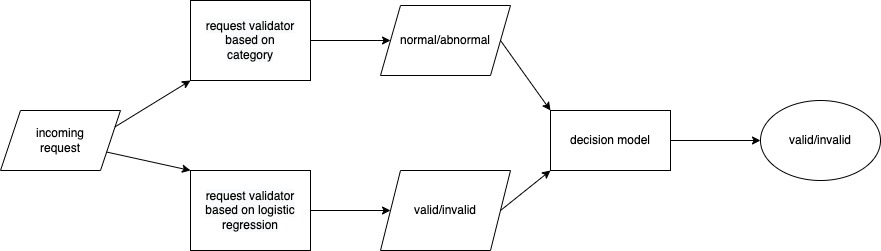
\includegraphics[width=\linewidth, height=10cm,keepaspectratio]{figures/architecture.jpg}
   \caption{Malicious request validator architecture}
\end{figure}
result: When two prediction is the same, the result is straight forward. When the logistic regression model decided that the request is malicious, but the CNN model predicted the request is nornal, the CNN is favored. Otherwise, the Regression model classified the request as valid but the CNN predicted as abnormal, we'll favor the Regression. The desicion model can be expressed in a decision table:


\begin{table}
\begin{center}
\begin{tabular}{||c c c ||} 
 \hline
 Regression & CNN & Result  \\ [0.5ex] 
 \hline\hline
 Valid & Normal & Valid \\ 
 
 Valid & Abnormal & Valid  \\

 Invalid & Normal & Valid  \\
 
 Invalid & Abnormal & Invalid  \\ [1ex] 
\hline
\end{tabular}
\end{center}
\caption{\label{demo-table}Table 4.1}
\end{table}

The CNN validator will run for a set period of time (usually one or two weeks) to collect the familiar category of incoming requests and assign a threshold (which can be the mean or maximum (if we are optimistic) distance between each request vector in the observing stage and the sum vector). The same will also happened with the Regression model. After that training phase, the module will run on 'active phase', parallel with the WAF. 
\begin{itemize}
    \item  To predict whether a request is malicious or not.
\end{itemize}
Our architecture is described in Figure 14 below, suggest a reasonable decision model for the combination of CNN and the Regression model
\begin{figure}[!h]
     \centering
     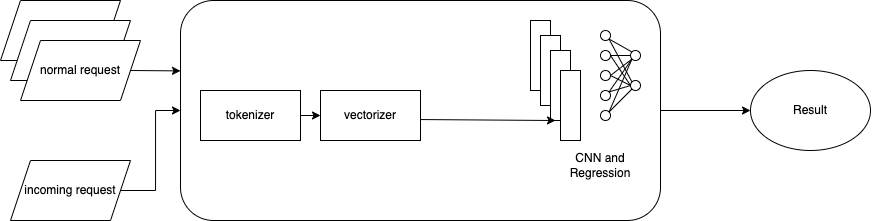
\includegraphics[width=\linewidth, height=10cm,keepaspectratio]{figures/architecture 2.drawio.png}
   \caption{Decision model for the combination of CNN and the Regression model}
\end{figure}
\newpage
The request is routed through the module, which predicts the category. The category of suspicious request is then compared with the common category. Then the Regression model will determined whether the request is good or bad, combining with the normal or abnormal status to decide the result. 
